\section{Results}

  For each of the signal regions, the total expectation  and observed yields are shown in Tables~\ref{table:yield_EMu},~\ref{table:yield_SF} and ~\ref{table:yield_all} for respectively the $e\mu$ channel, same-flavor channels
  and, moreover, for all the channels combined. When calculating the total expect yields, the $t\bar{t}$, DY, diboson and $t\bar{t}Z$ scale factors as well as their uncertainties are taken into account. 
  The uncertainties related to MC statistics, pile-up, jet energy scale, top-$\pt$ reweighting, trigger efficiencies, lepton identification and isolation scale factors, $b$-tagging scale factors
  and the different background components are also included.
  The observed yields and its statistically are also visually presented in Figures~\ref{fig:signalRegions-emu},~\ref{fig:signalRegions-sf} and~\ref{fig:signalRegions-all} where, additionally, three
  signal mass configurations are overlaid. The uncertainty band includes the MC statistics, pile-up, jet energy scale, top-$\pt$ reweighting, trigger efficiencies, lepton identification and isolation scale factors, $b$-tagging scale factors
  uncertainties.
  The observation is in agreement with the prediction within uncertainties.

  \begin{sidewaystable}
    \centering
    \setlength{\tabcolsep}{4pt}
    \footnotesize
    \begin{tabular}{l|cc|cccccccc|ccccc} 
  \rotatebox[origin=c]{50}{signal region} & \rotatebox[origin=c]{50}{observed} & \rotatebox[origin=c]{50}{expected}&\rotatebox[origin=c]{50}{MC stat}&\rotatebox[origin=c]{50}{PU}&\rotatebox[origin=c]{50}{JEC}&\rotatebox[origin=c]{50}{top-\pt}&\rotatebox[origin=c]{50}{trigger}&\rotatebox[origin=c]{50}{lepton SF}&\rotatebox[origin=c]{50}{b-tag SF-b}&\rotatebox[origin=c]{50}{b-tag SF-l}&\rotatebox[origin=c]{50}{TTJets}&\rotatebox[origin=c]{50}{TTZ}&\rotatebox[origin=c]{50}{multiBoson}&\rotatebox[origin=c]{50}{TTXNoZ}&\rotatebox[origin=c]{50}{DY} \\ 
  \hline 
 $0$  & 40 & 27.80 & 1.35 & 0.77 & 1.06 & 0.46 & 0.05 & 0.04 & 0.05 & 0.01 & 26.78 $\pm$ 13.39 & 0.17 $\pm$ 0.04 & 0.34 $\pm$ 0.09 & 0.18 $\pm$ 0.05 & 0.0 $\pm$ 0.00 \\ 
 $1$  & 3 & 1.00 & 0.25 & 0.08 & 0.05 & 0.01 & 0.01 & 0.01 & 0.01 & 0.01 & 0.98 $\pm$ 0.50 & 0.02 $\pm$ 0.01 & 0.0 $\pm$ 0.00 & 0.0 $\pm$ 0.00 & 0.0 $\pm$ 0.00 \\ 
 $2$  & 18 & 13.24 & 0.89 & 0.21 & 0.06 & 0.14 & 0.02 & 0.02 & 0.02 & 0.02 & 12.42 $\pm$ 6.21 & 0.39 $\pm$ 0.08 & 0.11 $\pm$ 0.03 & 0.21 $\pm$ 0.06 & 0.0 $\pm$ 0.00 \\ 
 $3$  & 1 & 1.13 & 0.19 & 0.03 & 0.07 & 0.01 & 0.01 & 0.01 & 0.02 & 0.01 & 0.85 $\pm$ 0.43 & 0.05 $\pm$ 0.02 & 0.05 $\pm$ 0.02 & 0.13 $\pm$ 0.04 & 0.0 $\pm$ 0.00 \\ 
 $4$  & 0 & 0.06 & 0.03 & 0.01 & 0.01 & 0.01 & 0.01 & 0.01 & 0.01 & 0.00 & 0.03 $\pm$ 0.02 & 0.02 $\pm$ 0.01 & 0.0 $\pm$ 0.00 & 0.0 $\pm$ 0.01 & 0.0 $\pm$ 0.00 \\ 
 $5$  & 0 & 0.90 & 0.44 & 0.02 & 0.04 & 0.01 & 0.01 & 0.01 & 0.01 & 0.01 & 0.78 $\pm$ 0.39 & 0.1 $\pm$ 0.02 & 0.0 $\pm$ 0.00 & 0.03 $\pm$ 0.01 & 0.0 $\pm$ 0.00 \\ 
 $6$  & 0 & 0.12 & 0.07 & 0.01 & 0.01 & 0.01 & 0.01 & 0.01 & 0.01 & 0.01 & 0.1 $\pm$ 0.06 & 0.02 $\pm$ 0.01 & 0.0 $\pm$ 0.00 & 0.0 $\pm$ 0.00 & 0.0 $\pm$ 0.00 \\ 
 $7$  & 0 & 0.01 & 0.02 & 0.01 & 0.01 & 0.01 & 0.00 & 0.01 & 0.01 & 0.00 & 0.01 $\pm$ 0.01 & 0.0 $\pm$ 0.01 & 0.0 $\pm$ 0.00 & 0.0 $\pm$ 0.01 & 0.0 $\pm$ 0.00 \\ 
 $8$  & 0 & 0.48 & 0.12 & 0.01 & 0.02 & 0.02 & 0.01 & 0.01 & 0.01 & 0.01 & 0.27 $\pm$ 0.14 & 0.15 $\pm$ 0.03 & 0.0 $\pm$ 0.00 & 0.07 $\pm$ 0.02 & 0.0 $\pm$ 0.00 \\ 
 $9$  & 0 & 0.05 & 0.03 & 0.01 & 0.02 & 0.00 & 0.01 & 0.01 & 0.01 & 0.00 & 0.0 $\pm$ 0.00 & 0.01 $\pm$ 0.01 & 0.0 $\pm$ 0.00 & 0.04 $\pm$ 0.01 & 0.0 $\pm$ 0.00 \\ 
 $10$  & 1 & 0.18 & 0.07 & 0.02 & 0.02 & 0.01 & 0.01 & 0.01 & 0.01 & 0.01 & 0.04 $\pm$ 0.02 & 0.11 $\pm$ 0.03 & 0.01 $\pm$ 0.01 & 0.01 $\pm$ 0.01 & 0.0 $\pm$ 0.00 \\ 
 $11$  & 0 & 0.24 & 0.08 & 0.01 & 0.01 & 0.01 & 0.01 & 0.01 & 0.01 & 0.01 & 0.07 $\pm$ 0.04 & 0.11 $\pm$ 0.03 & 0.0 $\pm$ 0.00 & 0.07 $\pm$ 0.02 & 0.0 $\pm$ 0.00 \\ 
 $12$  & 0 & 0.05 & 0.02 & 0.01 & 0.01 & 0.00 & 0.01 & 0.01 & 0.01 & 0.00 & 0.0 $\pm$ 0.00 & 0.04 $\pm$ 0.01 & 0.0 $\pm$ 0.00 & 0.0 $\pm$ 0.01 & 0.0 $\pm$ 0.00 \\ 
\end{tabular} 

    \caption{Yields and uncertainties for the total background in each of the signal regions for the $e\mu$ channel. Scale factors are applied for the $t\bar{t}$, DY, diboson and $t\bar{t}Z$ backgrounds.}
    \label{table:yield_EMu}
  \end{sidewaystable}

  \begin{sidewaystable}
    \centering
    \footnotesize
    \setlength{\tabcolsep}{4pt}
    \begin{tabular}{l|cc|cccccccc|ccccc} 
  \rotatebox[origin=c]{50}{signal region} & \rotatebox[origin=c]{50}{observed} & \rotatebox[origin=c]{50}{expected}&\rotatebox[origin=c]{50}{MC stat}&\rotatebox[origin=c]{50}{PU}&\rotatebox[origin=c]{50}{JEC}&\rotatebox[origin=c]{50}{top-\pt}&\rotatebox[origin=c]{50}{trigger}&\rotatebox[origin=c]{50}{lepton SF}&\rotatebox[origin=c]{50}{b-tag SF-b}&\rotatebox[origin=c]{50}{b-tag SF-l}&\rotatebox[origin=c]{50}{TTJets}&\rotatebox[origin=c]{50}{TTZ}&\rotatebox[origin=c]{50}{multiBoson}&\rotatebox[origin=c]{50}{TTXNoZ}&\rotatebox[origin=c]{50}{DY} \\ 
  \hline 
 $0$  & 27 & 28.48 & 1.05 & 0.75 & 0.73 & 0.45 & 0.09 & 0.01 & 0.02 & 0.02 & 27.27 $\pm$ 13.64 & 0.26 $\pm$ 0.06 & 0.07 $\pm$ 0.02 & 0.24 $\pm$ 0.06 & 0.67 $\pm$ 0.17 \\ 
 $1$  & 3 & 1.98 & 0.58 & 0.03 & 0.09 & 0.01 & 0.01 & 0.01 & 0.01 & 0.01 & 1.72 $\pm$ 0.87 & 0.04 $\pm$ 0.01 & 0.06 $\pm$ 0.02 & 0.03 $\pm$ 0.01 & 0.08 $\pm$ 0.03 \\ 
 $2$  & 17 & 14.89 & 0.87 & 0.39 & 0.57 & 0.15 & 0.03 & 0.02 & 0.03 & 0.03 & 13.5 $\pm$ 6.75 & 0.47 $\pm$ 0.10 & 0.33 $\pm$ 0.09 & 0.2 $\pm$ 0.05 & 0.16 $\pm$ 0.05 \\ 
 $3$  & 2 & 2.01 & 0.28 & 0.05 & 0.04 & 0.02 & 0.01 & 0.01 & 0.02 & 0.01 & 1.63 $\pm$ 0.82 & 0.08 $\pm$ 0.02 & 0.06 $\pm$ 0.02 & 0.07 $\pm$ 0.02 & 0.13 $\pm$ 0.04 \\ 
 $4$  & 0 & 0.09 & 0.03 & 0.01 & 0.04 & 0.01 & 0.00 & 0.01 & 0.00 & 0.01 & 0.04 $\pm$ 0.02 & 0.03 $\pm$ 0.01 & 0.0 $\pm$ 0.00 & 0.01 $\pm$ 0.01 & 0.01 $\pm$ 0.01 \\ 
 $5$  & 1 & 0.60 & 0.14 & 0.03 & 0.05 & 0.02 & 0.01 & 0.01 & 0.01 & 0.01 & 0.45 $\pm$ 0.23 & 0.08 $\pm$ 0.02 & 0.01 $\pm$ 0.01 & 0.06 $\pm$ 0.02 & 0.0 $\pm$ 0.00 \\ 
 $6$  & 0 & 0.26 & 0.07 & 0.01 & 0.01 & 0.01 & 0.01 & 0.01 & 0.01 & 0.01 & 0.05 $\pm$ 0.03 & 0.04 $\pm$ 0.01 & 0.07 $\pm$ 0.02 & 0.04 $\pm$ 0.02 & 0.01 $\pm$ 0.01 \\ 
 $7$  & 0 & 0.12 & 0.05 & 0.02 & 0.01 & 0.00 & 0.00 & 0.01 & 0.01 & 0.01 & 0.0 $\pm$ 0.00 & 0.02 $\pm$ 0.01 & 0.02 $\pm$ 0.01 & 0.01 $\pm$ 0.01 & 0.06 $\pm$ 0.02 \\ 
 $8$  & 2 & 0.53 & 0.15 & 0.00 & 0.00 & 0.01 & 0.01 & 0.01 & 0.02 & 0.01 & 0.04 $\pm$ 0.02 & 0.2 $\pm$ 0.05 & 0.1 $\pm$ 0.03 & 0.07 $\pm$ 0.02 & 0.04 $\pm$ 0.02 \\ 
 $9$  & 0 & 0.47 & 0.21 & 0.03 & 0.02 & 0.00 & 0.01 & 0.01 & 0.02 & 0.01 & 0.0 $\pm$ 0.00 & 0.04 $\pm$ 0.01 & 0.1 $\pm$ 0.03 & 0.06 $\pm$ 0.02 & 0.21 $\pm$ 0.06 \\ 
 $10$  & 1 & 0.23 & 0.06 & 0.01 & 0.16 & 0.01 & 0.01 & 0.01 & 0.01 & 0.01 & 0.08 $\pm$ 0.05 & 0.1 $\pm$ 0.03 & 0.0 $\pm$ 0.01 & 0.05 $\pm$ 0.02 & 0.01 $\pm$ 0.01 \\ 
 $11$  & 0 & 0.73 & 0.26 & 0.07 & 0.15 & 0.01 & 0.01 & 0.01 & 0.01 & 0.04 & 0.0 $\pm$ 0.00 & 0.12 $\pm$ 0.03 & 0.35 $\pm$ 0.09 & 0.03 $\pm$ 0.01 & 0.01 $\pm$ 0.01 \\ 
 $12$  & 0 & 0.18 & 0.05 & 0.01 & 0.01 & 0.01 & 0.01 & 0.01 & 0.01 & 0.01 & 0.02 $\pm$ 0.03 & 0.07 $\pm$ 0.02 & 0.0 $\pm$ 0.00 & 0.06 $\pm$ 0.02 & 0.03 $\pm$ 0.01 \\ 
\end{tabular} 

    \caption{Yields and uncertainties for the total background in each of the signal regions for the same-flavor ($ee/\mu\mu$) channels. Scale factors are applied for the $t\bar{t}$, DY, diboson and $t\bar{t}Z$ backgrounds.}
    \label{table:yield_SF}
  \end{sidewaystable}
 
  \begin{sidewaystable}
    \centering
    \footnotesize
    \setlength{\tabcolsep}{4pt}
    \begin{tabular}{l|cc|cccccccc|ccccc} 
  \rotatebox[origin=c]{50}{signal region} & \rotatebox[origin=c]{50}{observed} & \rotatebox[origin=c]{50}{expected}&\rotatebox[origin=c]{50}{MC stat}&\rotatebox[origin=c]{50}{PU}&\rotatebox[origin=c]{50}{JEC}&\rotatebox[origin=c]{50}{top-\pt}&\rotatebox[origin=c]{50}{trigger}&\rotatebox[origin=c]{50}{lepton SF}&\rotatebox[origin=c]{50}{b-tag SF-b}&\rotatebox[origin=c]{50}{b-tag SF-l}&\rotatebox[origin=c]{50}{TTJets}&\rotatebox[origin=c]{50}{TTZ}&\rotatebox[origin=c]{50}{multiBoson}&\rotatebox[origin=c]{50}{TTXNoZ}&\rotatebox[origin=c]{50}{DY} \\ 
  \hline 
 $0$  & 67 & 56.28 & 1.70 & 1.52 & 1.79 & 0.91 & 0.13 & 0.04 & 0.03 & 0.03 & 54.05 $\pm$ 27.03 & 0.43 $\pm$ 0.09 & 0.41 $\pm$ 0.11 & 0.42 $\pm$ 0.11 & 0.67 $\pm$ 0.17 \\ 
 $1$  & 6 & 2.98 & 0.63 & 0.11 & 0.04 & 0.01 & 0.01 & 0.01 & 0.01 & 0.01 & 2.71 $\pm$ 1.36 & 0.06 $\pm$ 0.02 & 0.06 $\pm$ 0.02 & 0.03 $\pm$ 0.01 & 0.08 $\pm$ 0.03 \\ 
 $2$  & 35 & 28.13 & 1.24 & 0.59 & 0.63 & 0.29 & 0.04 & 0.01 & 0.02 & 0.04 & 25.91 $\pm$ 12.96 & 0.86 $\pm$ 0.18 & 0.45 $\pm$ 0.12 & 0.41 $\pm$ 0.11 & 0.16 $\pm$ 0.05 \\ 
 $3$  & 3 & 3.14 & 0.34 & 0.07 & 0.03 & 0.03 & 0.01 & 0.02 & 0.03 & 0.01 & 2.47 $\pm$ 1.24 & 0.13 $\pm$ 0.03 & 0.11 $\pm$ 0.03 & 0.2 $\pm$ 0.05 & 0.13 $\pm$ 0.04 \\ 
 $4$  & 0 & 0.15 & 0.05 & 0.02 & 0.04 & 0.01 & 0.01 & 0.01 & 0.01 & 0.01 & 0.07 $\pm$ 0.04 & 0.05 $\pm$ 0.01 & 0.0 $\pm$ 0.00 & 0.02 $\pm$ 0.01 & 0.01 $\pm$ 0.01 \\ 
 $5$  & 1 & 1.50 & 0.46 & 0.02 & 0.01 & 0.03 & 0.01 & 0.01 & 0.01 & 0.01 & 1.23 $\pm$ 0.62 & 0.17 $\pm$ 0.04 & 0.01 $\pm$ 0.01 & 0.09 $\pm$ 0.03 & 0.0 $\pm$ 0.00 \\ 
 $6$  & 0 & 0.37 & 0.10 & 0.01 & 0.01 & 0.01 & 0.01 & 0.01 & 0.01 & 0.01 & 0.15 $\pm$ 0.08 & 0.05 $\pm$ 0.02 & 0.07 $\pm$ 0.02 & 0.04 $\pm$ 0.02 & 0.01 $\pm$ 0.01 \\ 
 $7$  & 0 & 0.14 & 0.05 & 0.02 & 0.01 & 0.01 & 0.00 & 0.01 & 0.01 & 0.01 & 0.01 $\pm$ 0.01 & 0.02 $\pm$ 0.01 & 0.02 $\pm$ 0.01 & 0.01 $\pm$ 0.01 & 0.06 $\pm$ 0.02 \\ 
 $8$  & 2 & 1.00 & 0.19 & 0.01 & 0.02 & 0.02 & 0.01 & 0.02 & 0.02 & 0.01 & 0.3 $\pm$ 0.16 & 0.35 $\pm$ 0.07 & 0.1 $\pm$ 0.03 & 0.13 $\pm$ 0.04 & 0.04 $\pm$ 0.02 \\ 
 $9$  & 0 & 0.52 & 0.21 & 0.03 & 0.01 & 0.00 & 0.01 & 0.01 & 0.02 & 0.01 & 0.0 $\pm$ 0.00 & 0.05 $\pm$ 0.01 & 0.1 $\pm$ 0.03 & 0.1 $\pm$ 0.03 & 0.21 $\pm$ 0.06 \\ 
 $10$  & 2 & 0.41 & 0.09 & 0.02 & 0.15 & 0.01 & 0.01 & 0.01 & 0.01 & 0.01 & 0.12 $\pm$ 0.06 & 0.22 $\pm$ 0.05 & 0.01 $\pm$ 0.01 & 0.06 $\pm$ 0.02 & 0.01 $\pm$ 0.01 \\ 
 $11$  & 0 & 0.97 & 0.27 & 0.08 & 0.16 & 0.01 & 0.01 & 0.01 & 0.01 & 0.04 & 0.07 $\pm$ 0.04 & 0.23 $\pm$ 0.05 & 0.35 $\pm$ 0.09 & 0.1 $\pm$ 0.03 & 0.01 $\pm$ 0.01 \\ 
 $12$  & 0 & 0.22 & 0.05 & 0.01 & 0.01 & 0.01 & 0.01 & 0.01 & 0.01 & 0.01 & 0.02 $\pm$ 0.03 & 0.12 $\pm$ 0.03 & 0.0 $\pm$ 0.00 & 0.06 $\pm$ 0.02 & 0.03 $\pm$ 0.01 \\ 
\end{tabular} 

    \caption{Yields and uncertainties for the total background in each of the signal regions for all channels combined. Scale factors are applied for the $t\bar{t}$, DY, diboson and $t\bar{t}Z$ backgrounds.}
    \label{table:yield_all}
  \end{sidewaystable}


  % and in Figures~\ref{fig:signalRegions-emu}-\ref{fig:signalRegions-all}.
  \begin{figure}
    \centering
    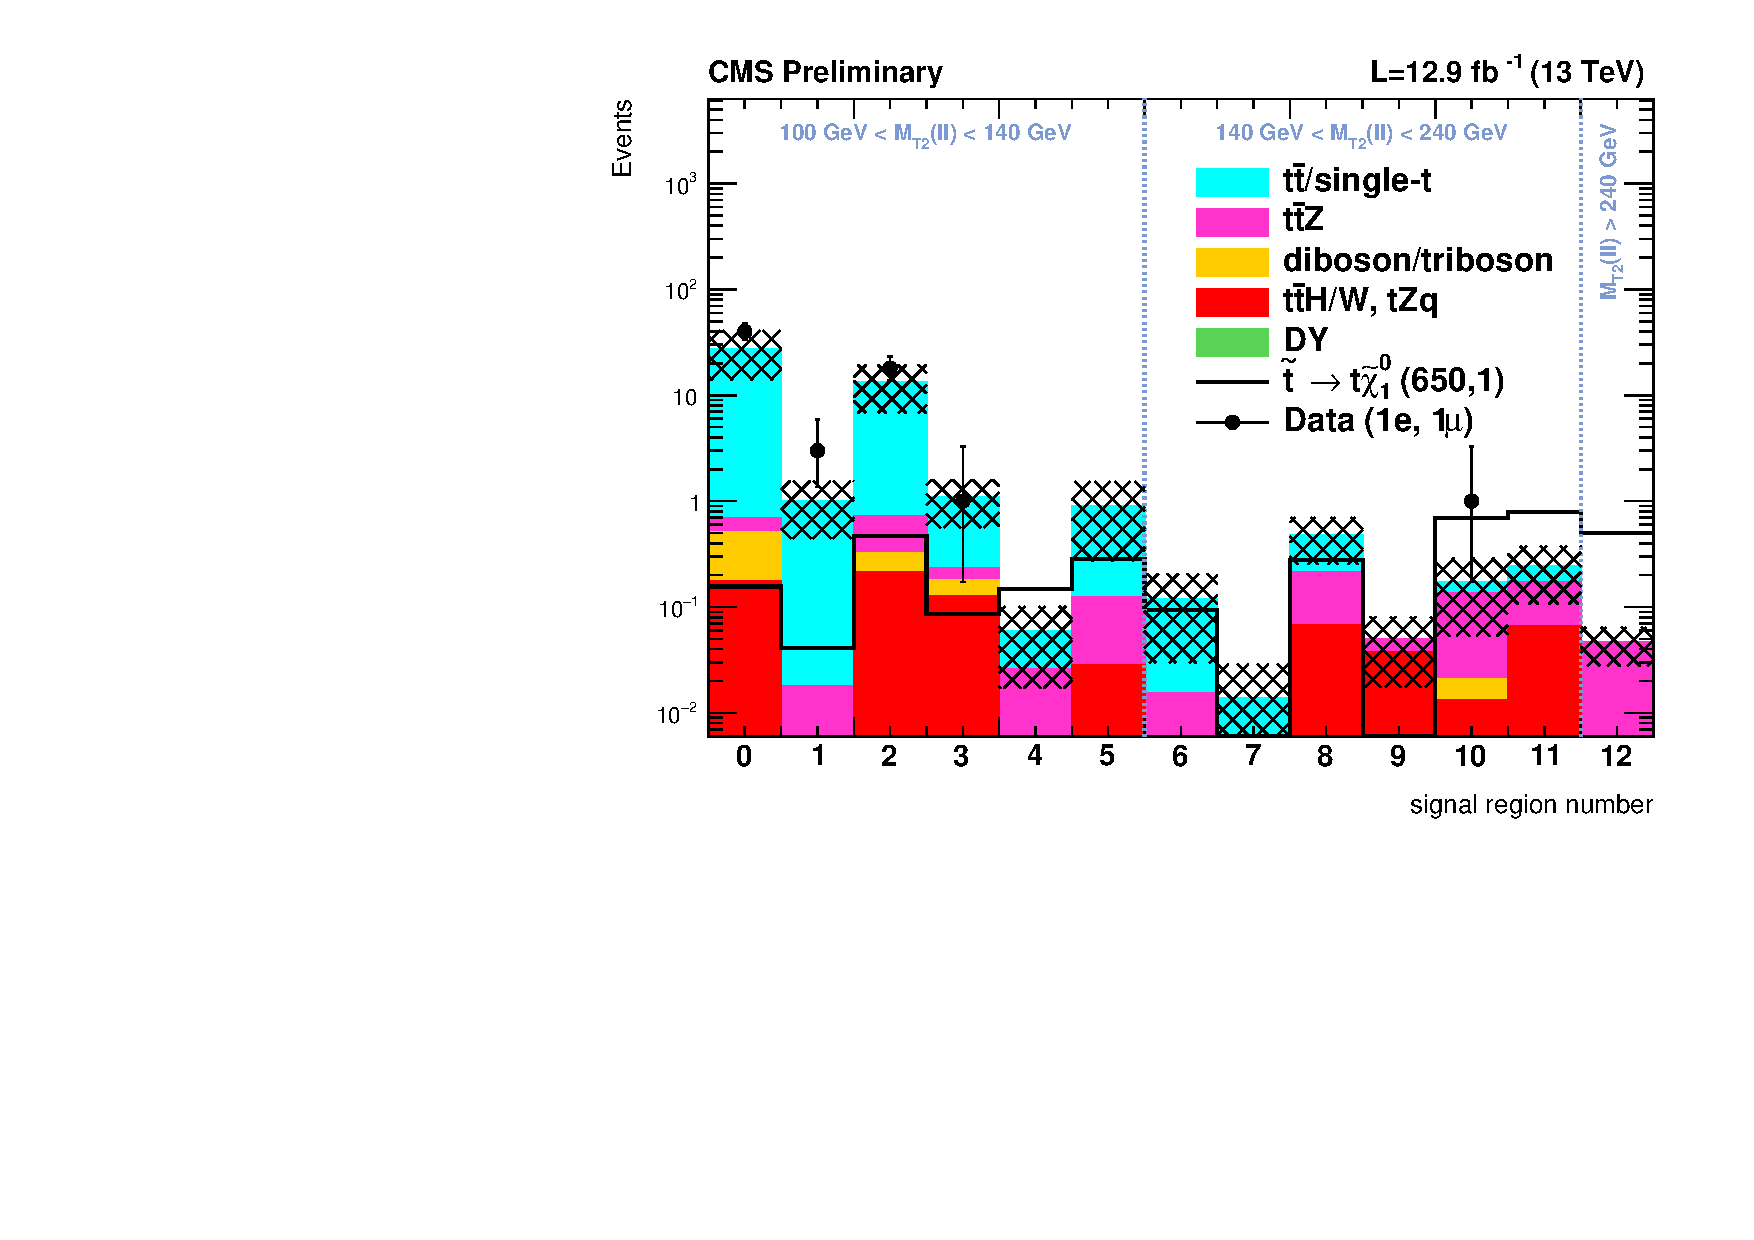
\includegraphics[width=0.9\textwidth]{figures/regions80X/DY-DD/TTZ-DD-Top16009/TTJets-DD/multiBoson-DD/EMu_bkgs.pdf}
    \caption{Signal and background contributions in the signal regions, in the $e\mu$ channel. Scale factors are applied for the $t\bar{t}$, DY, diboson and $t\bar{t}Z$ backgrounds.}
    \label{fig:signalRegions-emu}
  \end{figure}

  \begin{figure}
    \centering
    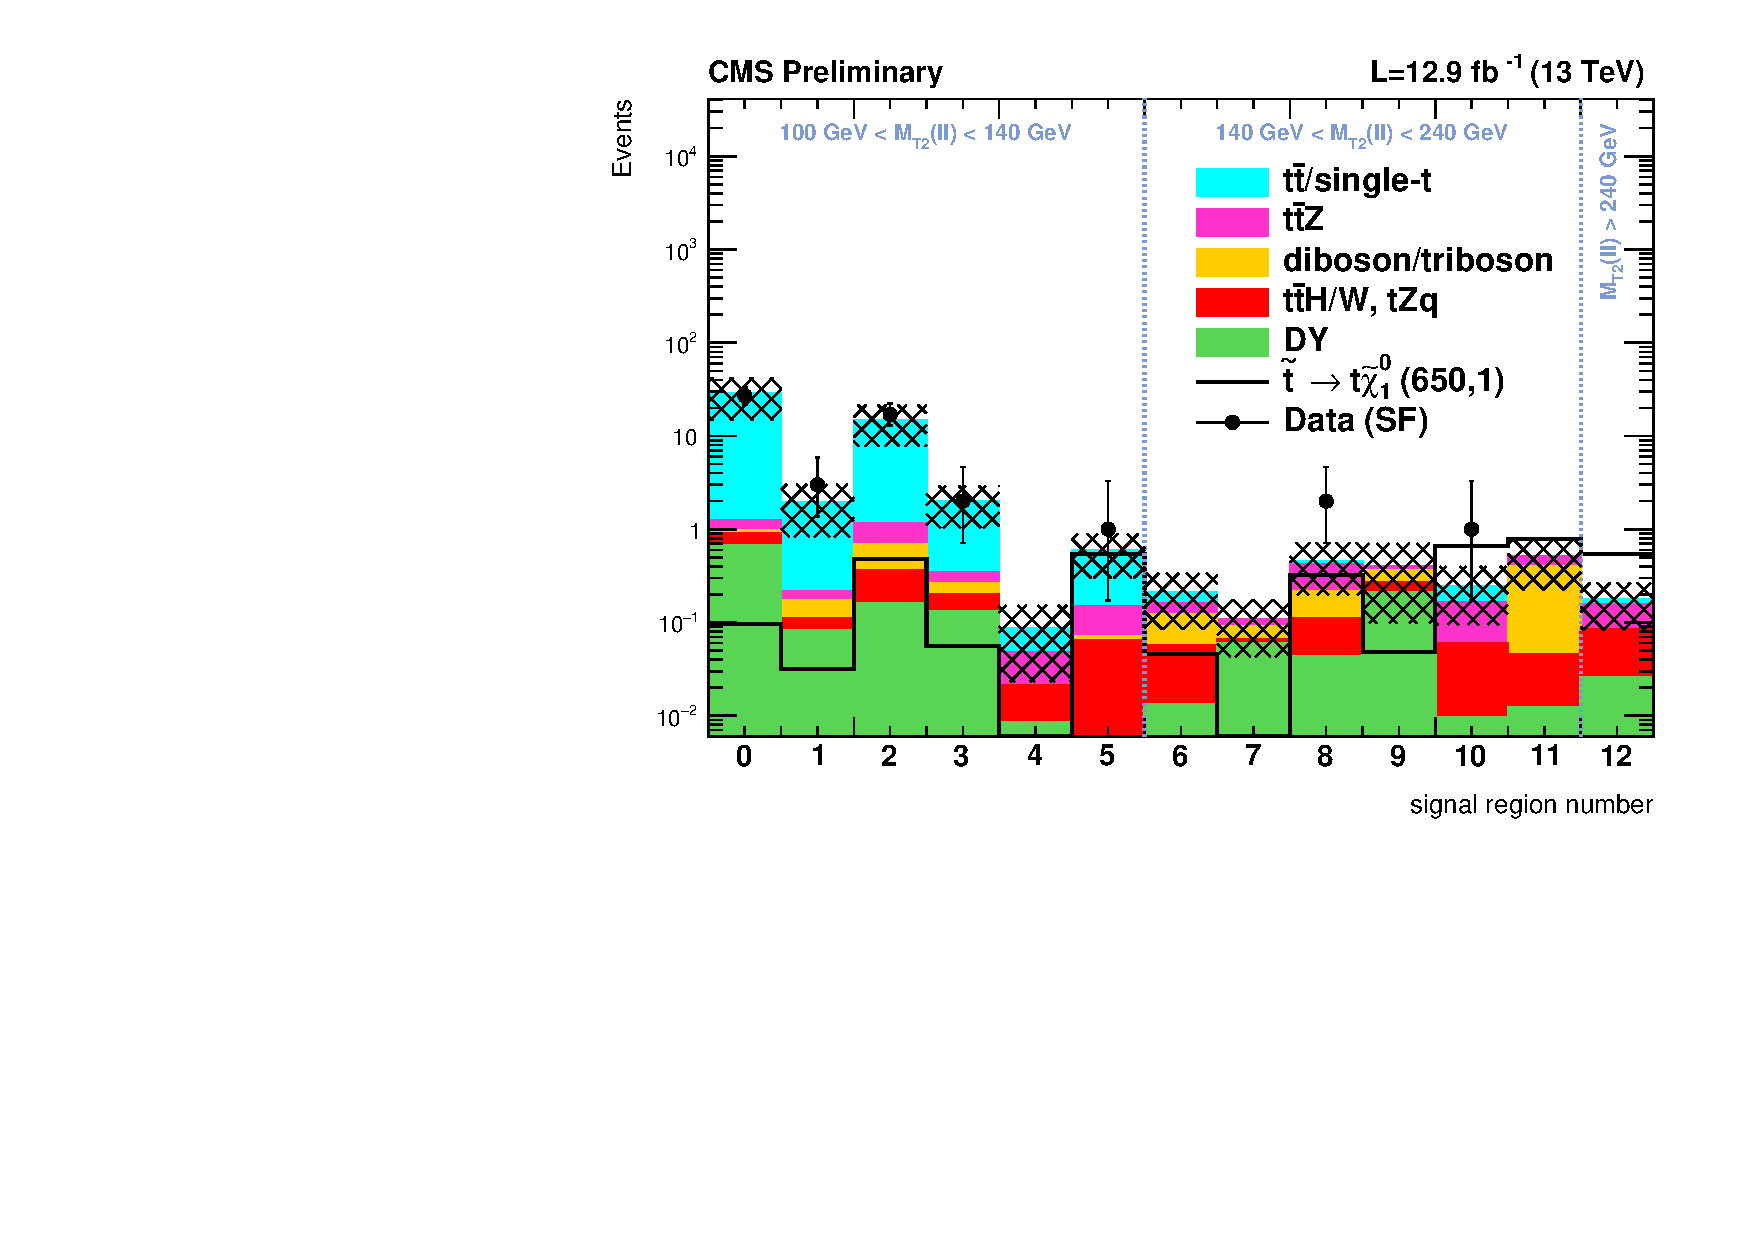
\includegraphics[width=0.9\textwidth]{figures/regions80X/DY-DD/TTZ-DD-Top16009/TTJets-DD/multiBoson-DD/SF_bkgs.pdf}
    \caption{Signal and background contributions in the signal regions, for the same-flavor channels ($ee$ and $\mu\mu$ combined). Scale factors are applied for the $t\bar{t}$, DY, diboson and $t\bar{t}Z$ backgrounds.}
    \label{fig:signalRegions-sf}
  \end{figure} 

  \begin{figure}
    \centering
    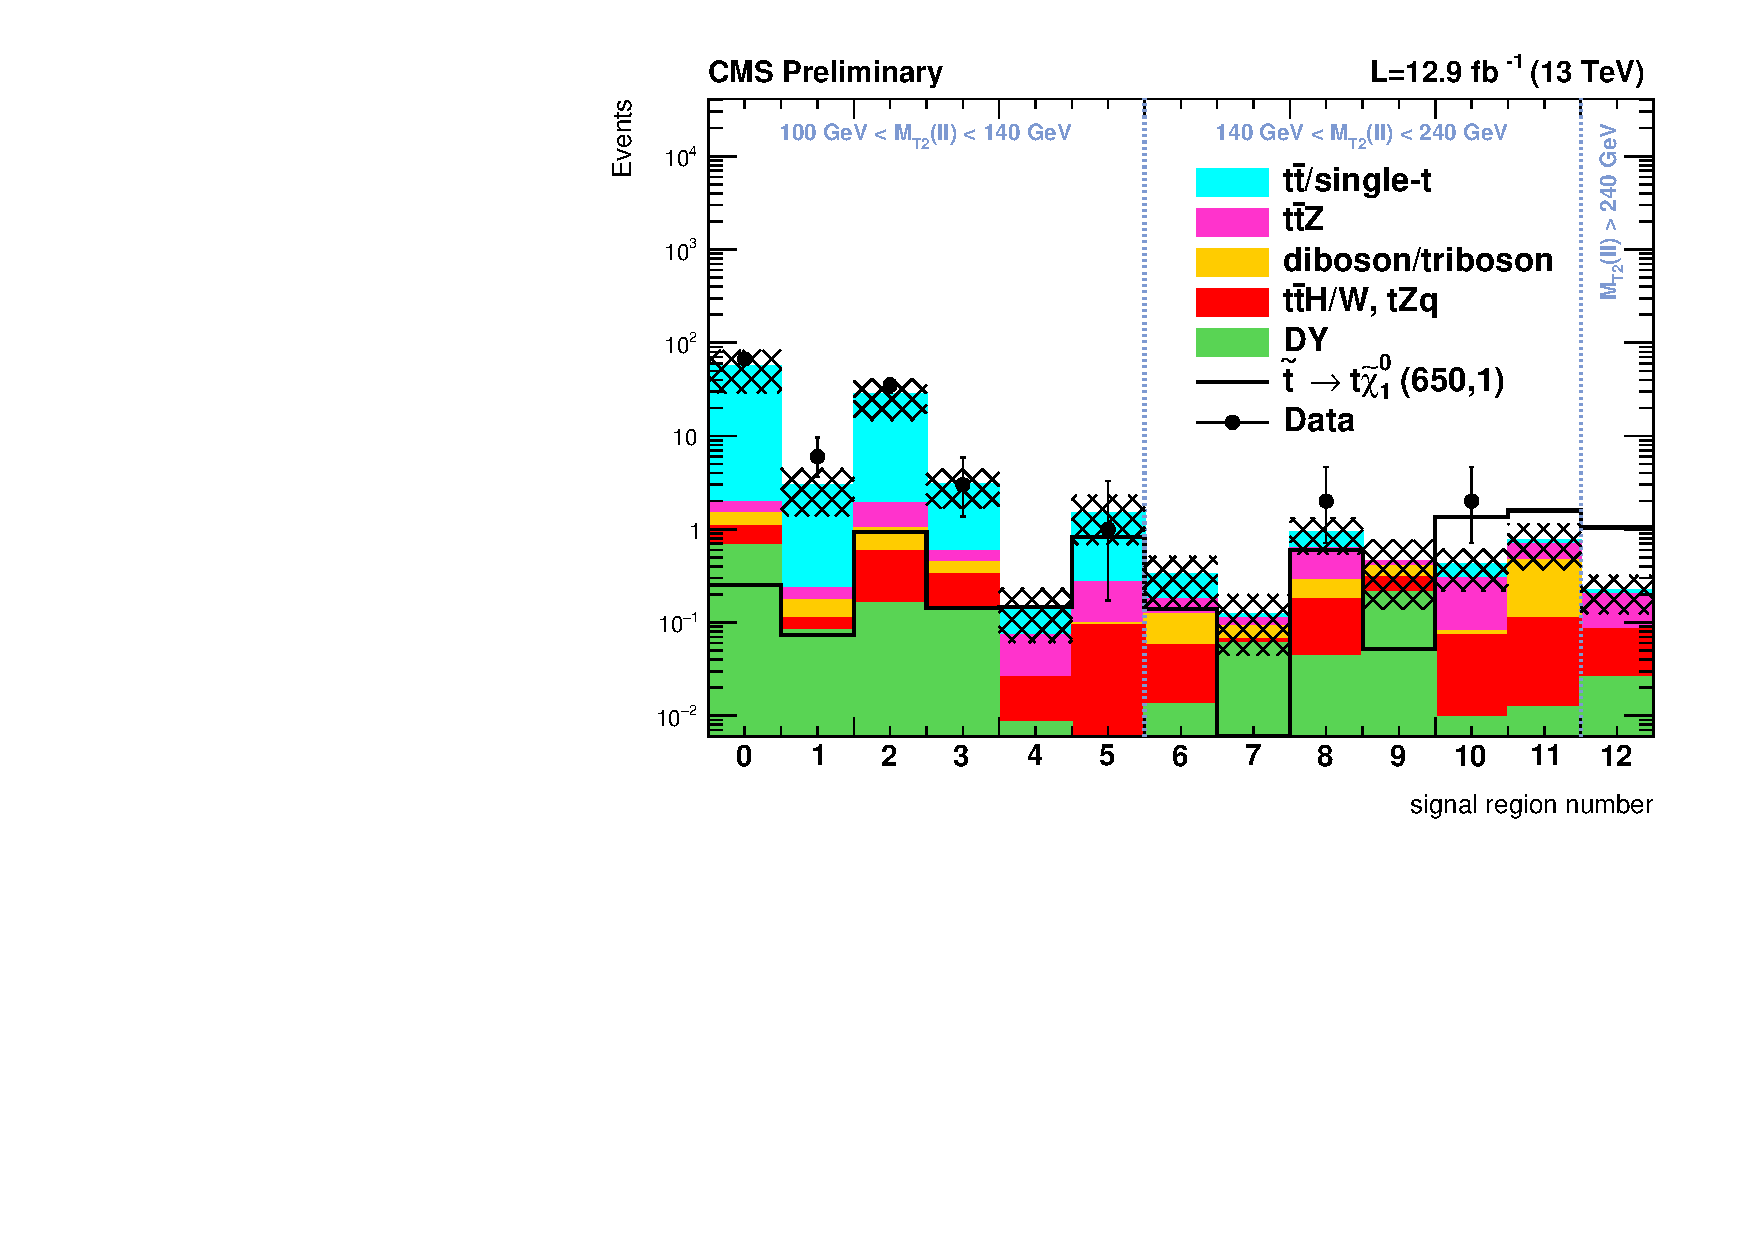
\includegraphics[width=0.9\textwidth]{figures/regions80X/DY-DD/TTZ-DD-Top16009/TTJets-DD/multiBoson-DD/all_bkgs.pdf}
    \caption{Signal and background contributions in the signal regions, for all channels combined. Scale factors are applied for the $t\bar{t}$, DY, diboson and $t\bar{t}Z$ backgrounds.}
    \label{fig:signalRegions-all}
  \end{figure}

  \begin{table}[ht]
  \begin{center}
  \caption{Expected limits for scalar models.}\label{limit_S_exp}
  \begin{tabular}{cc|ccccccccc} 
 & & \multicolumn{9}{c}{$m_\phi$ (GeV)} \\ 
& &10 & 15 & 20 & 50 & 95 & 100 & 200 & 300 & 500\\ 
 \hline \hline 
\multirow{3}{*}{$m_\chi$ (GeV)} & 1 & 0.84 &  & 1.17 & 1.01 &  & 1.93 & 4.05 & 8.66 & 38.62\\ 
 & 10 & 32.12 & 36.62 &  & 1.12 &  & 1.90 &  &  & \\ 
 & 50 & 218.25 &  &  & 195.62 & 93.62 &  & 4.42 & 8.78 & \\ 
 \end{tabular}
  \end{center}
  \end{table}

  \begin{table}[ht]
  \begin{center}
  \caption{Observed limits for scalar models.}\label{limit_S_obs}
  \begin{tabular}{cc|ccccccccc} 
 & & \multicolumn{9}{c}{$m_\phi$ (GeV)} \\ 
& &10 & 15 & 20 & 50 & 95 & 100 & 200 & 300 & 500\\ 
 \hline \hline 
\multirow{3}{*}{$m_\chi$ (GeV)} & 1 & 1.62 &  & 1.01 & 1.56 &  & 2.30 & 4.80 & 10.49 & 43.37\\ 
 & 10 & 45.94 & 62.24 &  & 1.16 &  & 2.37 &  &  & \\ 
 & 50 & 263.58 &  &  & 246.26 & 108.85 &  & 5.04 & 10.73 & \\ 
 \end{tabular}
  \end{center}
  \end{table}

  \begin{table}[ht]
  \begin{center}
  \caption{Expected limits for pseudo-scalar models.}\label{limit_PS_exp}
  \begin{tabular}{cc|ccccccccc} 
 & & \multicolumn{9}{c}{$m_\phi$ (GeV)} \\ 
& &10 & 15 & 20 & 50 & 95 & 100 & 200 & 300 & 500\\ 
 \hline \hline 
\multirow{3}{*}{$m_\chi$ (GeV)} & 1 & 1.99 &  & 1.74 & 2.01 &  & 2.57 & 3.67 & 5.86 & 40.62\\ 
 & 10 & 33.12 & 29.38 &  & 2.21 &  & 2.56 &  &  & \\ 
 & 50 & 142.25 &  &  & 135.25 & 38.81 &  & 3.73 & 5.83 & \\ 
 \end{tabular}
  \end{center}
  \end{table}

  \begin{table}[ht]
  \begin{center}
  \caption{Observed limits for pseudo-scalar models.}\label{limit_PS_obs}
  \begin{tabular}{cc|ccccccccc} 
 & & \multicolumn{9}{c}{$m_\phi$ (GeV)} \\ 
& &10 & 15 & 20 & 50 & 95 & 100 & 200 & 300 & 500\\ 
 \hline \hline 
\multirow{3}{*}{$m_\chi$ (GeV)} & 1 & 2.61 &  & 2.40 & 2.37 &  & 2.95 & 4.55 & 7.04 & 47.16\\ 
 & 10 & 43.66 & 34.58 &  & 2.79 &  & 3.08 &  &  & \\ 
 & 50 & 180.95 &  &  & 174.52 & 49.89 &  & 4.71 & 7.03 & \\ 
 \end{tabular}

  \end{center}
  \end{table}

  Using the above yields and uncertainties, we compute 95\% confidence level (CL) upper limits on the new physics cross section using the CLs method.
  Expected and observed limits for scalar and pseudoscalar models are shown in Tab.~\ref{limit_S_exp}--Tab.~\ref{limit_PS_obs}.

